
\section{Reasignación}
\index{asignación}
\index{sentencia!de asignación}
\index{reasignación}

Como habrás descubierto, es legal hacer más de una
asignación a la misma variable.  Una nueva asignación hace que una variable existente
se refiera a un nuevo valor (y deje de referirse al valor antiguo).

\begin{Verbatim}[frame=single]
>>> x = 5
>>> x
  5
>>> x = 7
>>> x
  7
\end{Verbatim}
%
La primera vez que mostramos
\texttt{x}, su valor es 5; la segunda vez, su
valor es 7.

La Figura~\ref{fig.assign2} muestra cómo se ve una \textbf{reasignación}
en un diagrama de estado. \index{diagrama!de estado} \index{estado, diagrama de}

En este punto quiero abordar un origen común de
confusión.
Debido a que Python utiliza el signo igual (\texttt{=}) para la asignación, es
tentador interpretar una sentencia del tipo \texttt{a = b} como una
proposición
matemática de igualdad, es decir, la afirmación de que \texttt{a} y
\texttt{b} son iguales.  Sin embargo, esta interpretación es incorrecta.
\index{igualdad y asignación}

Primero, la igualdad es una relación simétrica y la asignación no lo es.  Por
ejemplo, en matemáticas, si $a=7$ entonces $7=a$.  Pero en Python, la
sentencia \texttt{a = 7} es legal y \texttt{7 = a} no lo es.

Además, en matemáticas, una proposición de igualdad es verdadera o
falsa todo el tiempo.  Si $a=b$ ahora, entonces $a$ siempre será igual a $b$.
En Python, una sentencia de asignación puede igualar dos variables, pero
no tienen que permanecer iguales:

\begin{Verbatim}[frame=single]
>>> a = 5
>>> b = a    # a y b son iguales ahora
>>> a = 3    # a y b ya no son iguales
>>> b
  5
\end{Verbatim}
%
La tercera línea cambia el valor de \texttt{a} pero no cambia el
valor de \texttt{b}, por lo que ya no son iguales.

La reasignación de variables es a menudo útil, pero deberías utilizarla
con precaución.  Si los valores de las variables cambian frecuentemente, puede
hacer que el código sea difícil de leer y depurar.

\begin{figure}[t]
\begin{center}
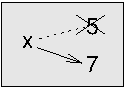
\includegraphics[width=0.25\textwidth]{images/assign2.pdf}
\end{center}
\caption{Reasignación de la variable \texttt{x}}
\label{fig.assign2}
\end{figure}



\hypertarget{update}{%
\section{Actualización de variables}\label{update}}

\index{actualización} \index{variable!actualización}

Uno de los usos habituales de las sentencias de asignación consiste en
realizar una actualización sobre una variable -- en la cual el valor
nuevo de esa variable depende del antiguo.

\begin{Verbatim}[frame=single]
x = x + 1
\end{Verbatim}

Esto quiere decir ''toma el valor actual de \texttt{x}, añádele 1, y luego actualiza \texttt{x} con el nuevo valor''.

Si intentas actualizar una variable que no existe, obtendrás un error,
ya que Python evalúa el lado derecho antes de asignar el valor a
\texttt{x}:

\begin{Verbatim}[frame=single]
>>> x = x + 1
  NameError: name 'x' is not defined
\end{Verbatim}

Antes de que puedas actualizar una variable, debes \emph{inicializarla},
normalmente mediante una simple asignación:

\index{inicialización (antes de actualizar)}

\begin{Verbatim}[frame=single]
>>> x = 0
>>> x = x + 1
\end{Verbatim}

Actualizar una variable añadiéndole 1 se denomina \emph{incrementar};
restarle 1 recibe el nombre de \emph{decrementar} (o disminuir).

\index{incrementar} \index{decrementar}

\hypertarget{la-instrucción-while}{%
\section{\texorpdfstring{La instrucción
\texttt{while}}{La instrucción while}}\label{la-instrucción-while}}

\index{while, instrucción} \index{instrucción!while} \index{while, bucle}
\index{bucle!while} \index{iteración}

Los PCs se suelen utilizar a menudo para automatizar tareas repetitivas.
Repetir tareas idénticas o muy similares sin cometer errores es algo que
a las máquinas se les da bien y en cambio a las personas no. Como las
iteraciones resultan tan habituales, Python proporciona varias
características en su lenguaje para hacerlas más sencillas.

Una forma de iteración en Python es la sentencia \texttt{while}. He aquí
un programa sencillo que cuenta hacia atrás desde cinco y luego dice
``¡Despegue!''.

\begin{python}[frame=single]
n = 5
while n > 0:
    print(n)
    n = n - 1
print("Despegue!")
\end{python}

Casi se puede leer la sentencia \texttt{while} como si estuviera escrita
en inglés. Significa, ``Mientras \texttt{n} sea mayor que 0, muestra el
valor de \texttt{n} y luego reduce el valor de \texttt{n} en 1 unidad.
Cuando llegues a 0, sal de la sentencia \texttt{while} y muestra la
palabra \texttt{¡Despegue!}''

\index{flujo de ejecución}


El flujo de ejecución de la sentencia \texttt{while} esta representado en la Figura \ref{fig:while} y explicado
de un modo más formal como sigue:

\begin{enumerate}
\def\labelenumi{\arabic{enumi}.}
\item
  Se evalúa la condición, obteniendo verdadero o falso.
\item
  Si la condición es falsa, se sale de la sentencia \texttt{while} y se
  continúa la ejecución en la siguiente sentencia.
\item
  Si la condición es verdadera, se ejecuta el cuerpo del \texttt{while}
  y luego se vuelve al paso 1.
\end{enumerate}

\begin{figure}[h]
    \centering
    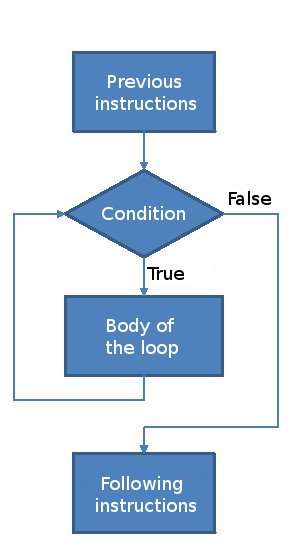
\includegraphics[width=0.25\textwidth]{images/while.jpg}
    \caption{Flujo del bucle while}
    \label{fig:while}
\end{figure}

Este tipo de flujo recibe el nombre de \emph{bucle}, ya que el tercer
paso enlaza de nuevo con el primero. Cada vez que se ejecuta el cuerpo
del bucle se dice que realizamos una \emph{iteración}. Para el bucle
anterior, podríamos decir que ``ha tenido cinco iteraciones'', lo que
significa que el cuerpo del bucle se ha ejecutado cinco veces.

\index{condición} \index{bucle} \index{cuerpo}

El cuerpo del bucle debe cambiar el valor de una o más variables, de
modo que la condición pueda en algún momento evaluarse como falsa y el
bucle termine. La variable que cambia cada vez que el bucle se ejecuta y
controla cuándo termina éste, recibe el nombre de \emph{variable de
iteración}. Si no hay variable de iteración, el bucle se repetirá para
siempre, resultando así un \emph{bucle infinito}.

Para entender como funcionas los bucles es una buena idea de hacer una traza donde, para cada iteración, escribimos los valores que tiene cada uno de las variables de iteración y resultados de otras acciones. Por ejemplo, considera el siguiente bucle:

\begin{python}[frame=single]
i = 1
while (i < 100):
    i = i * 2
    print (i)
\end{python}

Un ejemplo de una \emph{traza} esta en la Figura \ref{fig:traza}. Tenemos una columna para la condición, una columna por cada variable de iteración y otra columna más para la salida. Es una buena practica hacer esto con tus primeros bucles para entender cómo funcionan y ver que el valor de la variable de \verb|i| incrementa cada iteración hasta tener un valor mayor a 100 para que termina el bucle.

\begin{figure}[t]
    \centering
    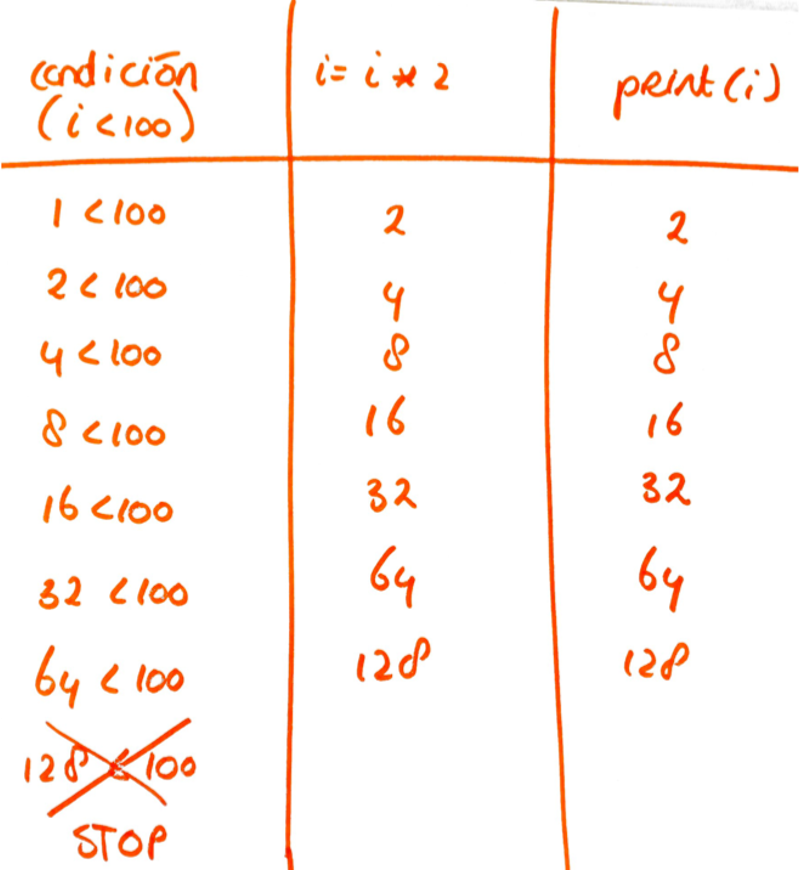
\includegraphics[width=0.4\textwidth]{images/traza.png}
    \caption{Traza de las iteraciones de un bucle}
    \label{fig:traza}
\end{figure}


Miramos otro ejemplo de un bucle:

\begin{python}[frame=single]
while (n != 1):
    print(n)
    if (n % 2) == 0:        #n es par
        n = n / 2
    else:                 #n es impar
        n = n*3 + 1
\end{python}
%
La condición para este bucle es \texttt{(\pythoninline{n} != 1)}, donde
\pythoninline{n} es la variable de iteración. El bucle continuará
hasta que \pythoninline{n} sea \pythoninline{1}, lo cual hace que la condición sea falsa.

En cada paso por el bucle, el programa muestra el valor de \pythoninline{n}
y luego verifica si es par o impar.  Si es par, \pythoninline{n} se
divide por 2.  Si es impar, el valor de \pythoninline{n} se reemplaza por
\pythoninline{n*3 + 1}. Por ejemplo, si el argumento pasado a \emph{sucesión}
es 3, los valores resultantes de \pythoninline{n} son 3, 10, 5, 16, 8, 4, 2, 1.

Dado que \pythoninline{n} a veces aumenta y a veces disminuye, no hay
demostración obvia de que \pythoninline{n} alcanzará el 1 alguna vez, o de que el programa
termina.  Para algunos valores particulares de \pythoninline{n}, podemos probar que
termina.  Por ejemplo, si el valor inicial es una potencia de dos,
\pythoninline{n} será par cada vez que se pase por el bucle
hasta que alcance el 1. El ejemplo anterior termina con tal sucesión,
comenzando con 16.
\index{Collatz, conjetura de}\index{conjetura de Collatz}

La pregunta difícil es si podemos probar que este programa termina
para {\em todos} los valores positivos de \pythoninline{n}.  Hasta ahora, ¡nadie ha
sido capaz de probarlo {\em o} refutarlo!  (Ver
  \url{http://en.wikipedia.org/wiki/Collatz_conjecture}.)


\begin{exercise}
Haz una traza de una ejecución del ultimo bucle para \pythoninline{(n = 16)}.
\end{exercise}



\hypertarget{bucles-infinitos}{%
\section{Bucles infinitos}\label{bucles-infinitos}}

Una fuente de diversión sin fin para los programadores es la
constatación de que las instrucciones del champú: ``Enjabone, aclare,
repita'', son un bucle infinito, ya que no hay una \emph{variable de
iteración} que diga cuántas veces debe ejecutarse el proceso.

\index{infinito, bucle} \index{bucle!infinito}

En el caso de una \texttt{cuenta\ atrás}, podemos verificar que el bucle
termina, ya que sabemos que el valor de \texttt{n} es finito, y podemos
ver que ese valor se va haciendo más pequeño cada vez que se repite el
bucle, de modo que en algún momento llegará a 0. Otras veces un bucle es
obviamente infinito, porque no tiene ninguna variable de iteración. Por ejemplo:

\begin{python}[frame=single]
i = 1
while (i < 10):
    print (i)
\end{python}

Es un bucle infinito, nunca parara de imprimir el mismo valor de \verb|i|.





\hypertarget{bucles-infinitos-y-break}{%
\section{\texorpdfstring{``Bucles infinitos'' y
\texttt{break}}{``Bucles infinitos'' y break}}\label{bucles-infinitos-y-break}}

\index{break, sentencia} \index{sentencia!break}

A veces no se sabe si hay que terminar un bucle hasta que se ha
recorrido la mitad del cuerpo del mismo. En ese caso se puede crear un
bucle infinito a propósito y usar la sentencia \texttt{break} para salir
fuera de él cuando se desee.

El bucle siguiente es, obviamente, un \emph{bucle infinito}, porque la
expresión lógica de la sentencia \texttt{while} es simplemente la
constante lógica \texttt{True\ (verdadero)};

\begin{python}[frame=single]
n = 10
while True:
    print(n)
    n = n - 1
print('Terminado!')
\end{python}

Si cometes el error de ejecutar este código, aprenderás rápidamente cómo
detener un proceso de Python bloqueado en el sistema, o tendrás que
localizar dónde se encuentra el botón de apagado de tu equipo. Este
programa funcionará para siempre, o hasta que la batería del equipo se
termine, ya que la expresión lógica al principio del bucle es siempre
cierta, en virtud del hecho de que esa expresión es precisamente el
valor constante \texttt{True}.

A pesar de que en este caso se trata de un bucle infinito inútil, se
puede usar ese diseño para construir bucles útiles, siempre que se tenga
la precaución de añadir código en el cuerpo del bucle para salir
explícitamente, usando \texttt{break} cuando se haya alcanzado la
condición de salida.

Por ejemplo, supón que quieres recoger entradas de texto del usuario
hasta que éste escriba \texttt{fin}. Podrías escribir:

\pythonexternal[frame=single]{code/copytildone1.py}

La condición del bucle es \texttt{True}, lo cual es verdadero siempre,
así que el bucle se repetirá hasta que se ejecute la sentencia break.

Cada vez que se entre en el bucle, se pedirá una entrada al usuario. Si
el usuario escribe \texttt{fin}, la sentencia \texttt{break} hará que se
salga del bucle. En cualquier otro caso, el programa repetirá cualquier
cosa que el usuario escriba y volverá al principio del bucle. Éste es un
ejemplo de su funcionamiento:

\begin{Verbatim}[frame=single]
> hola a todos
  hola a todos
> he terminado
  he terminado
> fin
  ¡Terminado!
\end{Verbatim}

Este modo de escribir bucles \texttt{while} es habitual, ya que así se
puede comprobar la condición en cualquier punto del bucle (no sólo al
principio), y se puede expresar la condición de parada afirmativamente
(``detente cuando ocurra\ldots{}''), en vez de tener que hacerlo con
lógica negativa (``sigue haciéndolo hasta que ocurra\ldots{}'').

\hypertarget{finalizar-iteraciones-con-continue}{%
\section{\texorpdfstring{Finalizar iteraciones con
\texttt{continue}}{Finalizar iteraciones con continue}}\label{finalizar-iteraciones-con-continue}}

\index{continue, sentencia} \index{sentencia!continue}

Algunas veces, estando dentro de un bucle se necesita terminar con la
iteración actual y saltar a la siguiente de forma inmediata. En ese caso
se puede utilizar la sentencia \texttt{continue} para pasar a la
siguiente iteración sin terminar la ejecución del cuerpo del bucle para
la actual.

A continuación se muestra un ejemplo de un bucle que repite lo que
recibe como entrada hasta que el usuario escribe ``fin'', pero trata las
líneas que empiezan por el carácter almohadilla como líneas que no deben
mostrarse en pantalla (algo parecido a lo que hace Python con los
comentarios).

\pythonexternal[frame=single]{code/copytildone2.py}

He aquí una ejecución de ejemplo de ese nuevo programa con la instrucción
\texttt{continue} añadida.

\begin{Verbatim}[frame=single]
> hola a todos
  hola a todos
> # no imprimas esto
> ¡imprime esto!
  ¡imprime esto!
> fin
  ¡Terminado!
\end{Verbatim}

Todas las líneas se imprimen en pantalla, excepto la que comienza con el
símbolo de almohadilla, ya que en ese caso se ejecuta \texttt{continue},
finaliza la iteración actual y salta de vuelta a la instrucción
\texttt{while} para comenzar la siguiente iteración, de modo que que se
omite la sentencia \texttt{print}.







\hypertarget{bucles-definidos-usando-for}{%
\section{\texorpdfstring{Bucles definidos usando
\texttt{for}}{Bucles definidos usando for}}\label{bucles-definidos-usando-for}}

\index{for, sentencia} \index{sentencia!for}

A veces se desea repetir un bucle a través de un \emph{serie} de cosas, como:

\begin{itemize}[nosep]
    \item un string (serie de caracteres), por ejemplo \verb|"abcdefghijklmnopqrstuvwxyz"|
    \item una lista, por ejemplo \pythoninline{["red", "orange", "yellow", "green"]}
   % \item las líneas de un archivo
    \item un rango de valores desde 1 hasta 10, por ejemplo  \pythoninline{range(1,11)}
\end{itemize}
Cuando se tiene una serie de cosas para recorrer, se puede
construir un bucle usando la instrucción \texttt{for} con \texttt{in}. 
La sintaxis de un bucle \texttt{for} es similar a la del
\texttt{while}, en ella hay una instrucción \pythoninline{for} y un cuerpo que se repite.


Un ejemplo para recorrer una cadena:

\begin{python}[frame=single]
for letra in "Hello":
    print(letra)
print('¡Terminado!')
\end{python}

El bucle \texttt{for} se mueve
recorriendo la cadena y ejecuta su cuerpo una vez para cada caracter en el string, produciendo esta salida:


\begin{Verbatim}[frame=single]
H
e
l
l
o
¡Terminado!
\end{Verbatim}

Un ejemplo para recorrer una lista:

\begin{python}[frame=single]
colores = ["red", "orange", "yellow", "green"]
for color in colores:
    print('Colors of the rainbow:', color)
print('¡Terminado!')
\end{python}

El bucle \texttt{for} se mueve
recorriendo la lista y ejecuta su cuerpo una vez para cada una de las
tres cadenas en la lista, produciendo esta salida:

\begin{Verbatim}[frame=single]
Colors of the rainbow: red
Colors of the rainbow: orange
Colors of the rainbow: yellow
Colors of the rainbow: green
¡Terminado!
\end{Verbatim}

La traducción de este bucle \texttt{for} al español no es tan directa
como en el caso del \texttt{while}, pero si piensas en los colores como
un \emph{conjunto}, sería algo así como: ``Ejecuta las instrucciones en el
cuerpo del bucle una vez \emph{para (for)} cada color que esté \emph{en
(in)} el conjunto llamado colores.''

Revisando el bucle \texttt{for}, \pythoninline{for} e \pythoninline{in} son palabras
reservadas de Python, mientras que \pythoninline{letra}, \pythoninline{color} y \pythoninline{colores} son
variables.

En concreto, \pythoninline{color} es la \emph{variable de iteración} para el
bucle for. La variable \pythoninline{color} cambia para cada iteración del
bucle y controla cuándo se termina el bucle \texttt{for}. La
\emph{variable de iteración} se desplaza sucesivamente a través de las
cuatro cadenas almacenadas en la variable \pythoninline{colores}.


A la instrucción \pythoninline{while} se la llama un bucle \emph{indefinido},
porque simplemente se repite hasta que cierta condición se hace
\texttt{Falsa}, mientras que el bucle \pythoninline{for} se la llama un bucle \emph{definido} porque se repite a través de
un conjunto conocido de elementos, de modo que ejecuta tantas
iteraciones como elementos hay en el conjunto.



%%%%

Recorrer los elementos de una lista 
con un ciclo \texttt{for} funciona bien si solo necesitas leer los elementos de la
lista.

\begin{Verbatim}[frame=single]
for queso in quesos:
    print(queso)
\end{Verbatim}
%

Pero si quieres escribir o actualizar los elementos,
necesitas los índices.  Una manera común de hacer eso es combinar
las funciones incorporadas \texttt{range} y \texttt{len}:
\index{bucle!con índices}
\index{indice@índice!bucle con}

\begin{python}[frame=single]
for i in range(len(numeros)):
    numeros[i] = numeros[i] * 2
\end{python}
%
Este bucle recorre la lista y actualiza cada elemento.  \texttt{len}
devuelve el número de elementos en la lista.  \texttt{range} devuelve
una lista de índices de 0 a $n-1$, donde $n$ es el largo de
la lista.  En cada paso por el bucle, \texttt{i} obtiene el índice
del siguiente elemento.  La sentencia de asignación en el cuerpo usa
\texttt{i} para leer el valor antiguo del elemento y asignar el
nuevo valor.
\index{actualizar!item@ítem}
\index{item@ítem!actualizar}

Un bucle \texttt{for} a través de una lista vacía nunca ejecuta el cuerpo:

\begin{python}[frame=single]
for x in []:
    print('Esto nunca ocurre.')
\end{python}
%
A pesar de que una lista puede contener otra lista, la lista
anidada aún cuenta como un solo elemento.  La longitud de esta lista es
cuatro:
\index{lista!anidada}
\index{anidada, lista}

\begin{Verbatim}[frame=single]
['spam', 1, ['Brie', 'Roquefort', 'Pol le Veq'], [1, 2, 3]]
\end{Verbatim}





\section{Range}\label{depuraciuxf3n}

La función \pythoninline{range} devuelve una serie o una secuencia de números y por eso es útil de usar con bucles \pythoninline{for} usando \pythoninline{in}. Por ejemplo:

\begin{python}[frame=single]
for i in range(2,5):
    print(i)
\end{python}

\begin{Verbatim}[frame=single]    
>>> %Run
2
3
4
\end{Verbatim}

Vemos que \pythoninline{range(inicio, fin)}
devuelve la serie de enteros desde \pythoninline{inicio} hasta \pythoninline{fin}–1.

Si no especificamos \pythoninline{inicio}, la serie empezará en 0.

\begin{python}[frame=single]
for i in range(4):
    print(i)
\end{python}

\begin{Verbatim}[frame=single]
>>> %Run    
0
1
2
3
\end{Verbatim}

También podemos especificar un incremento entre cada uno de los elementos de la serie con
\pythoninline{range(inicio, fin, inc)}. Devuelve la serie de enteros desde \pythoninline{inicio} hasta \pythoninline{fin}-1, tomando como incremento \pythoninline{inc}.

\begin{python}[frame=single]
for i in range(3,12,2):
    print(i)
\end{python}   

\begin{Verbatim}[frame=single]
>>> %Run
3
5
7
9
11
\end{Verbatim}

El incremento puede ser un numero negativo, para crear una serie que va de mayor a menor. Por ejemplo:

\begin{python}[frame=single]
>>> for i in range(6,1,-1):
    print(i)
\end{python}   

\begin{Verbatim}[frame=single]
>>> %Run
6
5
4
3
2
\end{Verbatim}



%%%%%%????????

\section{Más ejemplos: Recorrer las listas}
\label{filter}

Para sumar todos los números de una lista, puedes utilizar un bucle como este:

\begin{python}[frame=single]
def sumar_todos(t):
    total = 0
    for x in t:
        total += x
    return total
\end{python}

\index{operador!de actualización}
\index{actualización, operador de}
\index{aumentada, asignación}
\index{asignación!aumentada}

\texttt{total} se inicializa en 0.  En cada paso por el bucle,
\texttt{x} obtiene un elemento de la lista.  Recuerda que el operador 
\pythoninline{+=} proporciona una manera corta de actualizar una variable.  Esta
\textbf{ sentencia de asignación aumentada}:

\begin{Verbatim}[frame=single]
total += x
\end{Verbatim}
%
es equivalente a

\begin{Verbatim}[frame=single]
total = total + x
\end{Verbatim}
%
A medida que el bucle se ejecuta, \pythoninline{total} acumula la suma de los
elementos; una variable que se utiliza de esta manera a veces se llama
\textbf{ acumulador}.
\index{acumulador de suma}

Sumar los elementos de una lista es una operación tan común
que Python la facilita como función incorporada, \pythoninline{sum}:

\begin{Verbatim}[frame=single]
>>> t = [1, 2, 3]
>>> sum(t)
6
\end{Verbatim}
%
Una operación como esta que combina una secuencia de elementos en
un solo valor a veces se llama \textbf{ reducción}.
\index{patrón!de reducción}
\index{reducción, patrón de}
\index{recorrer}

A veces quieres recorrer una lista mientras construyes
otra.  Por ejemplo, la siguiente función toma una lista de cadenas
y devuelve una nueva lista que contiene cadenas que comienzan con mayúscula:

\begin{python}[frame=single]
def todas_con_mayuscula(t):
    res = []
    for s in t:
        res.append(s.capitalize())
    return res
\end{python}
%
la variable \pythoninline{res} se inicializa con una lista vacía; en cada paso por el bucle,
anexamos el elemento siguiente.  Entonces \pythoninline{res} es otro
tipo de acumulador.
\index{acumulador lista}

Una recorrido como la en \pythoninline{todas_con_mayuscula} a veces es llamada \textbf{
mapa} porque ``mapea'' una función (en este caso el método \pythoninline{capitalize}) sobre cada uno de los elementos en una secuencia.
\index{patrón!de mapa}
\index{mapa, patrón de}
\index{patrón!de filtro}
\index{filtro, patrón de}

Otra operación común es seleccionar algunos de los elementos de
una lista y devolver una sublista.  Por ejemplo, la siguiente
función toma una lista de cadenas y devuelve una lista que contiene
solo las cadenas escritas con mayúsculas:

\begin{python}[frame=single]
def solo_mayusculas(t):
    res = []
    for s in t:
        if s.isupper():
            res.append(s)
    return res
\end{python}
%
\pythoninline{isupper} es un método de cadena que devuelve \pythoninline{True} si
la cadena solo contiene letras mayúsculas.

Una recorrido como la en \pythoninline{solo_mayusculas} se llama \textbf{filtro} porque
selecciona algunos de los elementos y filtra los otros.

La mayoría de las operaciones de lista se pueden expresar como una combinación
de mapa, filtro y reducción.

%%%%%%%????????




\hypertarget{diseuxf1os-de-bucles}{%
\section{Diseños de bucles}\label{diseuxf1os-de-bucles}}

A menudo se usa un bucle \texttt{for} o \texttt{while} para movernos a
través de una lista de elementos o el contenido de un archivo y se busca
algo, como el valor más grande o el más pequeño de los datos que estamos
revisando.

Los bucles generalmente se construyen así:

\begin{itemize}[nosep]
\item
  Se inicializan una o más variables antes de que el bucle comience
\item
  Se realiza alguna operación con cada elemento en el cuerpo del bucle,
  posiblemente cambiando las variables dentro de ese cuerpo.
\item
  Se revisan las variables resultantes cuando el bucle se completa
\end{itemize}

Usaremos ahora una lista de números para demostrar los conceptos y
construcción de estos diseños de bucles.

\hypertarget{bucles-de-recuento-y-suma}{%
\subsection{Ejemplos: bucles de recuento y
suma}\label{bucles-de-recuento-y-suma}}

Por ejemplo, para contar el número de elementos en una lista, podemos
escribir el siguiente bucle \texttt{for}:

\begin{python}[frame=single]
contador = 0
for valor in [3, 41, 12, 9, 74, 15]:
    contador = contador + 1
print('Num. elementos: ', contador)
\end{python}

Ajustamos la variable \texttt{contador} a cero antes de que el bucle
comience, después escribimos un bucle \texttt{for} para movernos a
través de la lista de números. Nuestra variable de \emph{iteración} se
llama \texttt{valor}, y dado que no usamos \texttt{valor} dentro del
bucle, lo único que hace es controlar el bucle y hacer que el cuerpo del
mismo sea ejecutado una vez para cada uno de los valores de la lista.

En el cuerpo del bucle, añadimos 1 al valor actual de \texttt{contador}
para cada uno de los valores de la lista. Mientras el bucle se está
ejecutando, el valor de \texttt{contador} es la cantidad de valores que
se hayan visto ``hasta ese momento''.

Una vez el bucle se completa, el valor de \texttt{contador} es el número
total de elementos. El número total ``cae en nuestro poder'' al final
del bucle. Se construye el bucle de modo que obtengamos lo que queremos
cuando éste termina.

Otro bucle similar, que calcula el total de un conjunto de números, se
muestra a continuación:

\begin{python}[frame=single]
total = 0
for valor in [3, 41, 12, 9, 74, 15]:
    total = total + valor
print('Total: ', total)
\end{python}

En este bucle, \emph{sí} utilizamos la \emph{variable de iteración}. En
vez de añadir simplemente uno a \pythoninline{contador} como en el bucle
previo, ahora durante cada iteración del bucle añadimos el número actual
(3, 41, 12, etc.) al total en ese momento. Si piensas en la variable
\pythoninline{total}, ésta contiene la ``suma parcial de valores hasta ese
momento''. Así que antes de que el bucle comience, \pythoninline{total} es
cero, porque aún no se ha examinado ningún valor. Durante el bucle,
\pythoninline{total} es la suma parcial, y al final del bucle, \pythoninline{total}
es la suma total definitiva de todos los valores de la lista.

Cuando el bucle se ejecuta, \pythoninline{total} acumula la suma de los
elementos; una variable que se usa de este modo recibe a veces el nombre
de \emph{acumulador}.

\index{acumulador!sum}

Ni el bucle que cuenta los elementos ni el que los suma resultan
particularmente útiles en la práctica, dado que existen las funciones
internas \pythoninline{len()} y \pythoninline{sum()} que cuentan el número de
elementos de una lista y el total de elementos en la misma
respectivamente.

\hypertarget{bucles-de-muxe1ximos-y-muxednimos}{%
\subsection{Bucles de máximos y
mínimos}\label{bucles-de-muxe1ximos-y-muxednimos}}

\index{bucle!máximo} \index{bucle!mínimo} \index{None, valor especial}
\index{valor especial!None}

Para encontrar el valor mayor de una lista o secuencia, construimos el
bucle siguiente:

\begin{python}[frame=single]
mayor = None
print('Antes:', mayor)
for valor in [3, 41, 12, 9, 74, 15]:
    if (mayor is None) or (valor > mayor) :
        mayor = valor
    print('Bucle:', valor, mayor)
print('Despues mayor:', mayor)
\end{python}

Cuando se ejecuta el programa, se obtiene la siguiente salida:

\begin{Verbatim}[frame=single]
Antes: None
Bucle: 3 3
Bucle: 41 41
Bucle: 12 41
Bucle: 9 41
Bucle: 74 74
Bucle: 15 74
Despues mayor: 74
\end{Verbatim}

Debemos pensar en la variable \pythoninline{mayor} como el ``mayor valor visto
hasta ese momento''. Antes del bucle, asignamos a \pythoninline{mayor} el
valor \pythoninline{None}. \pythoninline{None} es un valor constante especial que se
puede almacenar en una variable para indicar que la variable está
``vacía''. Necesitamos la variable, pero no sabemos todavía que valor asignarle.

Antes de que el bucle comience, el mayor valor visto hasta entonces es
\pythoninline{None}, dado que no se ha visto aún ningún valor. Durante la
ejecución del bucle, si \pythoninline{mayor} es \pythoninline{None}, entonces
tomamos el primer valor que tenemos como el mayor hasta entonces. Se
puede ver en la primera iteración, cuando el valor de \pythoninline{valor} es
3, mientras que \pythoninline{mayor} es \pythoninline{None}, inmediatamente hacemos
que \pythoninline{mayor} pase a ser 3.

Tras la primera iteración, \pythoninline{mayor} ya no es \pythoninline{None}, así
que la segunda parte de la expresión lógica compuesta que comprueba si
\pythoninline{valor > mayor} se activará sólo cuando
encontremos un valor que sea mayor que el ``mayor hasta ese momento''.
Cuando encontramos un nuevo valor ``mayor aún'', tomamos ese nuevo valor
para \pythoninline{mayor}. Se puede ver en la salida del programa que
\pythoninline{mayor} pasa desde 3 a 41 y luego a 74.

Al final del bucle, se habrán revisado todos los valores y la variable
\pythoninline{mayor} contendrá entonces el mayor valor de la lista.

Para calcular el número más pequeño, el código es muy similar con un
pequeño cambio:

\begin{Verbatim}[frame=single]
print('Antes:', menor)
for valor in [3, 41, 12, 9, 74, 15]:
    if (menor is None) or (valor < menor):
        menor = valor
    print('Bucle:', valor, menor)
print('Despues menor:', menor)
\end{Verbatim}

De nuevo, \pythoninline{menor} es el ``menor hasta ese momento'' antes,
durante y después de que el bucle se ejecute. Cuando el bucle se ha
completado, \pythoninline{menor} contendrá el valor mínimo de la lista

También como en el caso del número de elementos y de la suma, las
funciones internas \pythoninline{max()} y \pythoninline{min()} convierten la
escritura de este tipo de bucles en innecesaria.



\section{Ejemplo: Calcular raíces cuadradas con bucles}
\label{squareroot}
\index{raiz cuadrada@raíz cuadrada}

Los bucles se utilizan a menudo en programas que calculan
resultados numéricos iniciando con una respuesta aproximada y
mejorándola iterativamente.
\index{metodo@método!de Newton}

Por ejemplo, una manera de calcular raíces cuadradas es el método de Newton.
Supongamos que quieres saber la raíz cuadrada de $a$.  Si comienzas
con casi cualquier estimación, $x$, puedes calcular una mejor
estimación con la siguiente fórmula:

\[ y = \frac{x + a/x}{2} \]
%
Por ejemplo, si $a$ es 4 y $x$ es 3:

\begin{Verbatim}[frame=single]
>>> a = 4
>>> x = 3
>>> y = (x + a/x) / 2
>>> y
  2.16666666667
\end{Verbatim}
%
El resultado está más cerca de la respuesta correcta ($\sqrt{4} = 2$).  Si
repetimos el proceso con una nueva estimación, se acerca aún más:

\begin{Verbatim}[frame=single]
>>> x = y
>>> y = (x + a/x) / 2
>>> y
  2.00641025641
\end{Verbatim}
%
Después de algunas actualizaciones más, la estimación es casi exacta:
\index{actualizar}

\begin{Verbatim}[frame=single]
>>> x = y
>>> y = (x + a/x) / 2
>>> y
  2.00001024003
>>> x = y
>>> y = (x + a/x) / 2
>>> y
  2.00000000003
\end{Verbatim}
%
En general, no sabemos de antemano cuántos pasos toma
llegar a la respuesta correcta, pero sabemos cuándo la obtenemos
porque la estimación
deja de cambiar:

\begin{Verbatim}[frame=single]
>>> x = y
>>> y = (x + a/x) / 2
>>> y
  2.0
>>> x = y
>>> y = (x + a/x) / 2
>>> y
  2.0
\end{Verbatim}
%
Cuando \texttt{y == x}, podemos parar.  Aquí hay un bucle que comienza
con una estimación inicial, \texttt{x}, y la mejora hasta que
deja de cambiar:

\begin{python}[frame=single]
while True:
    print(x)
    y = (x + a/x) / 2
    if y == x:
        break
    x = y
\end{python}
%
Para la mayoría de los valores de \texttt{a} esto funciona bien, pero en general es peligroso probar la igualdad de números \texttt{float}.
Los valores de coma flotante son solo aproximadamente correctos:
la mayoría de los números racionales, como $1/3$, y los números irracionales, como $\sqrt{2}$, no se pueden representar de manera exacta con un \texttt{float}.
\index{coma flotante}
\index{epsilon}

En lugar de verificar si \texttt{x} e \texttt{y} son exactamente iguales, es
más seguro utilizar la función \texttt{abs} para calcular el
valor absoluto, o magnitud, de la diferencia entre estos:

\begin{python}[frame=single]
epsilon = 0.0000001
while True:
    print(x)
    y = (x + a/x) / 2
    if (abs(y-x) < epsilon):
        break
    x = y
\end{python}

%
donde \pythoninline{epsilon} tiene un valor como \pythoninline{0.0000001} que
determina qué tan cerca es lo suficientemente cerca.






\hypertarget{depuraciuxf3n}{%
\section{Depuración}\label{depuraciuxf3n}}

\index{depuración}

A medida que vayas escribiendo programas más grandes, puede que notes
que vas necesitando emplear cada vez más tiempo en depurarlos. Más
código significa más oportunidades de cometer un error y más lugares
donde los bugs pueden esconderse.

\index{depuración!por bisección} \index{bisección, depuración por}

Un método para acortar el tiempo de depuración es ``depurar por
bisección''. Por ejemplo, si hay 100 líneas en tu programa y las
compruebas de una en una, te llevará 100 pasos.

En lugar de eso, intenta partir el problema por la mitad. Busca en medio
del programa, o cerca de ahí, un valor intermedio que puedas comprobar.
Añade una sentencia \texttt{print} (o alguna otra cosa que tenga un
efecto verificable), y haz funcionar el programa.

Si en el punto medio la verificación es incorrecta, el problema debería
estar en la primera mitad del programa. Si ésta es correcta, el problema
estará en la segunda mitad.

Cada vez que realices una comprobación como esta, reduces a la mitad el
número de líneas en las que buscar. Después de seis pasos (que son
muchos menos de 100), lo habrás reducido a una o dos líneas de código,
al menos en teoría.

En la práctica no siempre está claro qué es ``en medio del programa'', y
no siempre es posible colocar ahí una verificación. No tiene sentido
contar las líneas y encontrar el punto medio exacto. En lugar de eso,
piensa en lugares del programa en los cuales pueda haber errores y en
lugares donde resulte fácil colocar una comprobación. Luego elige un
sitio donde estimes que las oportunidades de que el bug esté por delante
y las de que esté por detrás de esa comprobación son más o menos las
mismas.

\hypertarget{glosario}{%
\section{Glosario}\label{glosario}}

\begin{description}
\item[acumulador]
Una variable usada en un bucle para sumar o acumular un resultado.
\end{description}

\index{acumulador}

\begin{description}
\item[bucle infinito]
Un bucle en el cual la condición de terminación no se satisface nunca o
para el cual no existe dicha condición de terminación.
\end{description}

\index{infinito, bucle} \index{bucle!infinito}

\begin{description}
\item[contador]
Una variable usada en un bucle para contar el número de veces que algo
sucede. Inicializamos el contador a cero y luego lo vamos incrementando
cada vez que queramos que ``cuente'' algo.
\end{description}

\index{contador}

\begin{description}
\item[decremento]
Una actualización que disminuye el valor de una variable.
\end{description}

\index{decremento}

\begin{description}
\item[inicializar]
Una asignación que da un valor inicial a una variable que va a ser
después actualizada.
\end{description}

\index{inicializar!variable}

\begin{description}
\tightlist
\item[incremento]
Una actualización que aumenta el valor de una variable (a menudo en una
unidad).
\end{description}

\index{incremento}

\begin{description}
\tightlist
\item[iteración]
Ejecución repetida de una serie de sentencias usando bien una función
que se llama a si misma o bien un bucle.
\end{description}


